\documentclass[tikz,border=6pt]{standalone}
\usepackage[T1]{fontenc}

\newcommand{\strike}[1]{\setbox0\hbox{#1}\rlap{\rule[0.55ex]{\wd0}{0.5pt}}#1}
\usetikzlibrary{decorations.pathreplacing,calc,positioning,arrows.meta}

\definecolor{prefixc}{RGB}{225,225,225}
\definecolor{templc}{RGB}{214,230,248}
\definecolor{wherec}{RGB}{253,231,206}
\definecolor{wheredark}{RGB}{250,206,160}
\definecolor{skipc}{RGB}{160,160,160}

\newcommand{\hh}{\textasciicircum\textasciicircum}

\begin{document}
% width of the code area, measured from the longest line, so the braces never
% overlap the code whatever font the document uses
\newlength{\codew}
\settowidth{\codew}{\ttfamily\footnotesize PREFIX table:  <http://csv2rdf.qlever.dev/table/>}
\pgfmathsetmacro{\W}{\codew/1cm + 0.35}
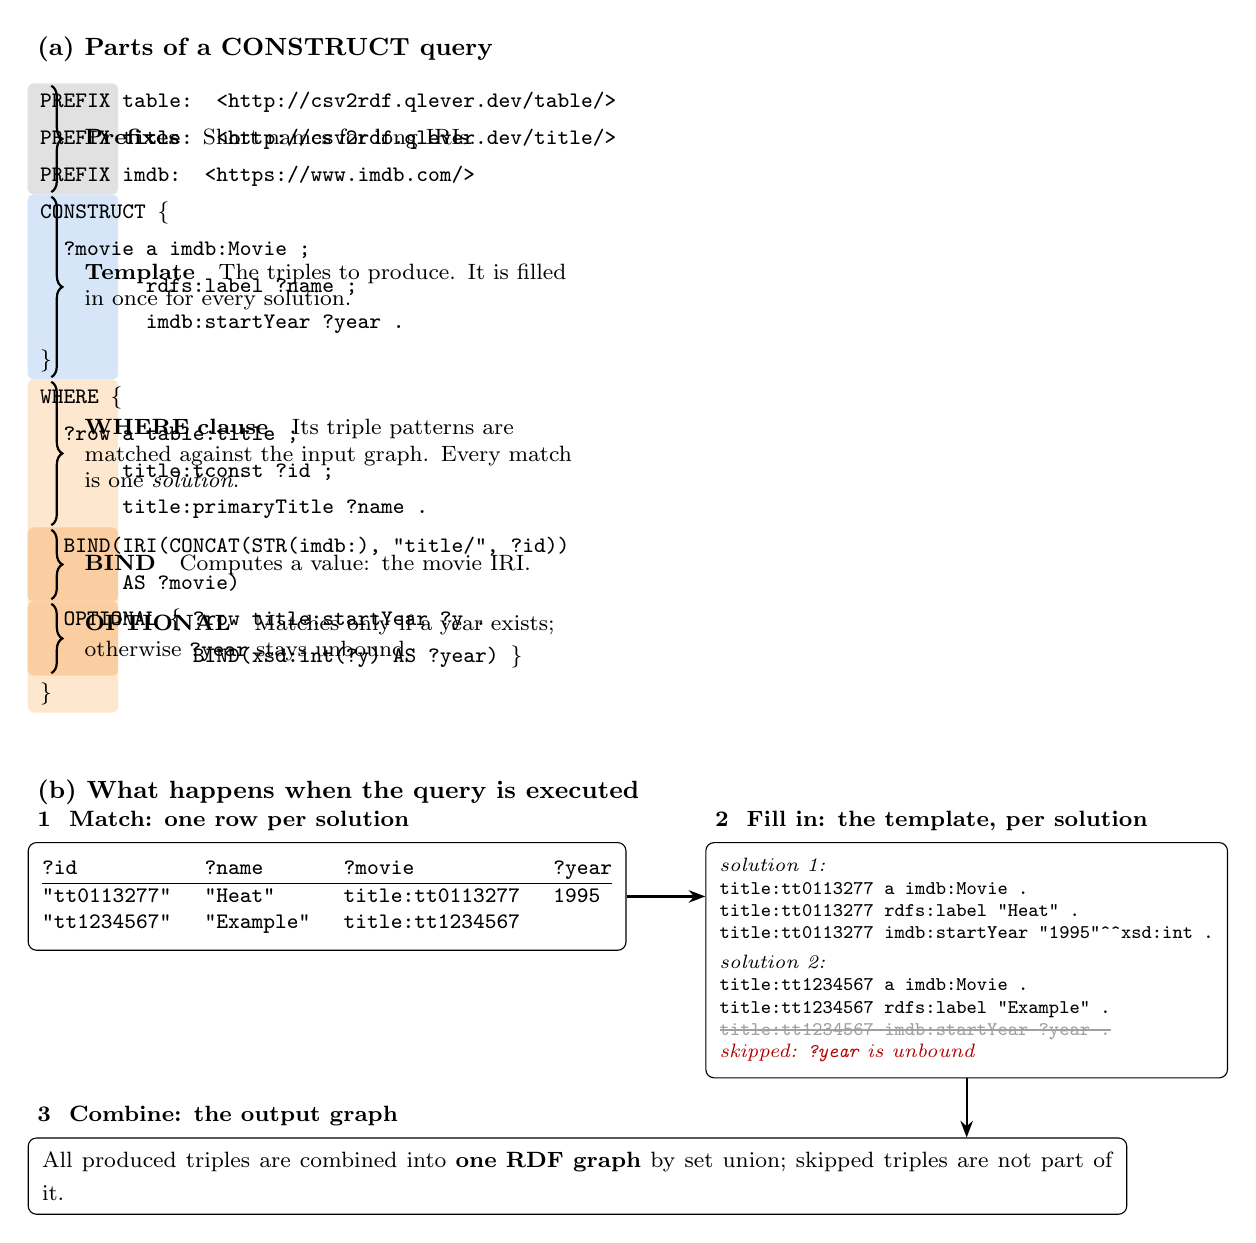
\begin{tikzpicture}[
  code/.style={anchor=west, font=\ttfamily\footnotesize, inner sep=0pt},
  note/.style={anchor=west, font=\footnotesize, text width=6.2cm, align=left},
  brace/.style={decorate, decoration={brace, amplitude=4pt}, thick},
  panel/.style={draw, rounded corners=3pt, fill=white, inner sep=5pt},
  title/.style={font=\footnotesize\bfseries, anchor=south west},
  arr/.style={-{Stealth[length=6pt]}, thick}
]
\def\lh{0.47}   % line height

% ---------- (a) background regions --------------------------------------
\newcommand{\region}[3]{%
  \fill[#3, rounded corners=2pt] (-0.15,{-(#1-1)*\lh+\lh/2}) rectangle (\W,{-(#2-1)*\lh-\lh/2});}
\region{1}{3}{prefixc}
\region{4}{8}{templc}
\region{9}{17}{wherec}
\region{13}{14}{wheredark}
\region{15}{16}{wheredark}

% ---------- (a) query lines ----------------------------------------------
\foreach \i/\t in {
 1/{PREFIX table: <http://csv2rdf.qlever.dev/table/>},
 2/{PREFIX title: <http://csv2rdf.qlever.dev/title/>},
 3/{PREFIX imdb:  <https://www.imdb.com/>},
 4/{CONSTRUCT \{},
 5/{\ \ ?movie a imdb:Movie ;},
 6/{\ \ \ \ \ \ \ \ \ rdfs:label ?name ;},
 7/{\ \ \ \ \ \ \ \ \ imdb:startYear ?year .},
 8/{\}},
 9/{WHERE \{},
 10/{\ \ ?row a table:title ;},
 11/{\ \ \ \ \ \ \ title:tconst ?id ;},
 12/{\ \ \ \ \ \ \ title:primaryTitle ?name .},
 13/{\ \ BIND(IRI(CONCAT(STR(imdb:), "title/", ?id))},
 14/{\ \ \ \ \ \ \ AS ?movie)},
 15/{\ \ OPTIONAL \{ ?row title:startYear ?y .},
 16/{\ \ \ \ \ \ \ \ \ \ \ \ \ BIND(xsd:int(?y) AS ?year) \}},
 17/{\}}}
{ \node[code] at (0,{-(\i-1)*\lh}) {\t}; }

% ---------- (a) annotations ----------------------------------------------
\newcommand{\annot}[4]{% from-line, to-line, bold label, text
  \draw[brace] (\W+0.15,{-(#1-1)*\lh+\lh/2-0.03}) -- (\W+0.15,{-(#2-1)*\lh-\lh/2+0.03});
  \node[note] at (\W+0.45,{-((#1+#2)/2-1)*\lh}) {\textbf{#3}\quad #4};}
\annot{1}{3}{Prefixes}{Short names for long IRIs.}
\annot{4}{8}{Template}{The triples to produce. It is filled in once for every solution.}
\annot{9}{12}{WHERE clause}{Its triple patterns are matched against the input graph. Every match is one \emph{solution}.}
\annot{13}{14}{BIND}{Computes a value: the movie IRI.}
\annot{15}{16}{OPTIONAL}{Matches only if a year exists; otherwise \texttt{?year} stays unbound.}

\node[font=\small\bfseries, anchor=south west] at (-0.15,\lh/2+0.15) {(a) Parts of a CONSTRUCT query};

% ---------- (b) evaluation ------------------------------------------------
\def\yb{-9.4}
\node[font=\small\bfseries, anchor=south west] at (-0.15,\yb+0.35) {(b) What happens when the query is executed};

% step 1: solutions
\node[panel, anchor=north west] (s1) at (-0.15,\yb) {%
  \footnotesize
  \begin{tabular}{@{}llll@{}}
    \texttt{?id} & \texttt{?name} & \texttt{?movie} & \texttt{?year}\\\hline
    \texttt{"tt0113277"} & \texttt{"Heat"} & \texttt{title:tt0113277} & \texttt{1995}\\
    \texttt{"tt1234567"} & \texttt{"Example"} & \texttt{title:tt1234567} & \textit{}\\
  \end{tabular}};
\node[title, anchor=south west] at ($(s1.north west)+(0,0.02)$) {\textbf{1\ \ Match:} one row per solution};

% step 2: instantiate
\node[panel, anchor=north west] (s2) at ($(s1.north east)+(1.0,0)$) {%
  \ttfamily\scriptsize
  \begin{tabular}{@{}l@{}}
    \textrm{\textit{solution 1:}}\\
    title:tt0113277 a imdb:Movie .\\
    title:tt0113277 rdfs:label "Heat" .\\
    title:tt0113277 imdb:startYear "1995"\hh{}xsd:int .\\[3pt]
    \textrm{\textit{solution 2:}}\\
    title:tt1234567 a imdb:Movie .\\
    title:tt1234567 rdfs:label "Example" .\\
    \textcolor{skipc}{\strike{title:tt1234567 imdb:startYear ?year .}}\\
    \textrm{\textit{\textcolor{red!70!black}{skipped: \texttt{?year} is unbound}}}\\
  \end{tabular}};
\node[title] at ($(s2.north west)+(0,0.02)$) {\textbf{2\ \ Fill in:} the template, per solution};

% step 3: union
\node[panel, anchor=north west, text width=13.6cm, align=left] (s3) at ($(s1.west |- s2.south)+(0,-0.75)$) {%
  \footnotesize All produced triples are combined into \textbf{one RDF graph} by set union; skipped triples are not part of it.};
\node[title] at ($(s3.north west)+(0,0.02)$) {\textbf{3\ \ Combine:} the output graph};

\draw[arr] (s1.east) -- (s1.east -| s2.west);
\draw[arr] (s2.south) -- (s2.south |- s3.north);
\end{tikzpicture}
\end{document}
% Here, the output graph contains five triples. As a graph is a set, a triple produced several times is contained in it only once, but the serialized output of an engine may still repeat it. Template triples without variables are copied into the output unchanged.